
\chapter{Binary Analysis: Support for the Analysis of Binary Executables}

\label{binaryAnalysis::overview}

\section{Introduction}

   ROSE supports the disassembly and analysis of binary executables for x86, PowerPC, and AMR
instruction sets.  ROSE implements this support as part of general research work
to support combining analysis for source code and analysis for binaries and supporting
performance analysis and optimization.  Through this support ROSE addresses the
requirements for the analysis and transformation of software in a general context useful
to as wide a group of users as possible.

   ROSE handles a number of binary executable file formats and also reads Dwarf information
into the AST to support additional analysis.

   Recent work in ROSE has added support for dynamic analysis and for mixing of dynamic
and static analysis using the Intel Pin framework. 
Intel Pin support in ROSE is presented in section~\ref{intel_pin}.

\section{The Binary AST}

\subsection{The Binary Executable Format}

    ROSE handles Linux and Windows binary formats; thus ELF format for Linux and PE, NE,
LE, DOS formats for Windows.  The details of each format are represented in IR nodes in
the AST (using structures common to the representation of such low level data).  About
60 IR nodes have been added to ROSE to support the binary executable formats; this
support allows the analysis of any Linux, Windows, OS\/2, or DOS binary executable.

   The binary executable file format can be analyzed separately from the instructions
using the command line option: {\tt -rose:read\_executable\_file\_format\_only}.  This
allows graphs generated using the ROSE visualization mechanisms (and even some analysis) 
to be easily restricted (in size) to the just the IR nodes specific to the binary
executable file format.

% \fixme{We need an example of the binary executable format AST.}

\begin{figure}
% \includegraphics[angle=90,scale=0.75,width=5in,height=1in]{\TopSourceDirectory/src/frontend/ExecFormats/BinaryFileFormat}
\includegraphics[angle=90,width=7.5in,height=8.5in]{\TopSourceDirectory/src/frontend/BinaryFormats/BinaryFileFormat}
\caption{The class design of the IR nodes for the binary file format.} 

\label{binaryAnalysis:BinaryExecutableFormatDesign}
\end{figure}

Figure \ref{binaryAnalysis:BinaryExecutableFormatDesign} shows the class design of the IR
nodes for the binary file format address the
requirements of ELF (Linux, and others), PE (MS Windows), NE (older MS Windows), 
LE (OS\/2), and DOS (MS Dos) executable formats.  The colors represent different
executable formats, brown classes are used as base classes for more than one
format. Dark colors represent principle IR nodes in the AST, lighter color IR nodes
represent supporting infrastructure in the AST.  Arrows are either dark colored or
light colored; dark colors represent class derivation, and light colors represent
member relationships.

% DQ (10/29/2008): Added documentation for file format (plus examples).
% This figure uses a saved (static) pdf file (not generated during the ``make docs'' rule).
% This was done because it is cropped using predefined pixel values which would not be
% easy to generate for a pdf that might be constantly changed.
\begin{figure}
% \includegraphics[angle=90,scale=0.75,width=5in,height=1in]{\TopSourceDirectory/src/frontend/ExecFormats/BinaryFileFormat}
% 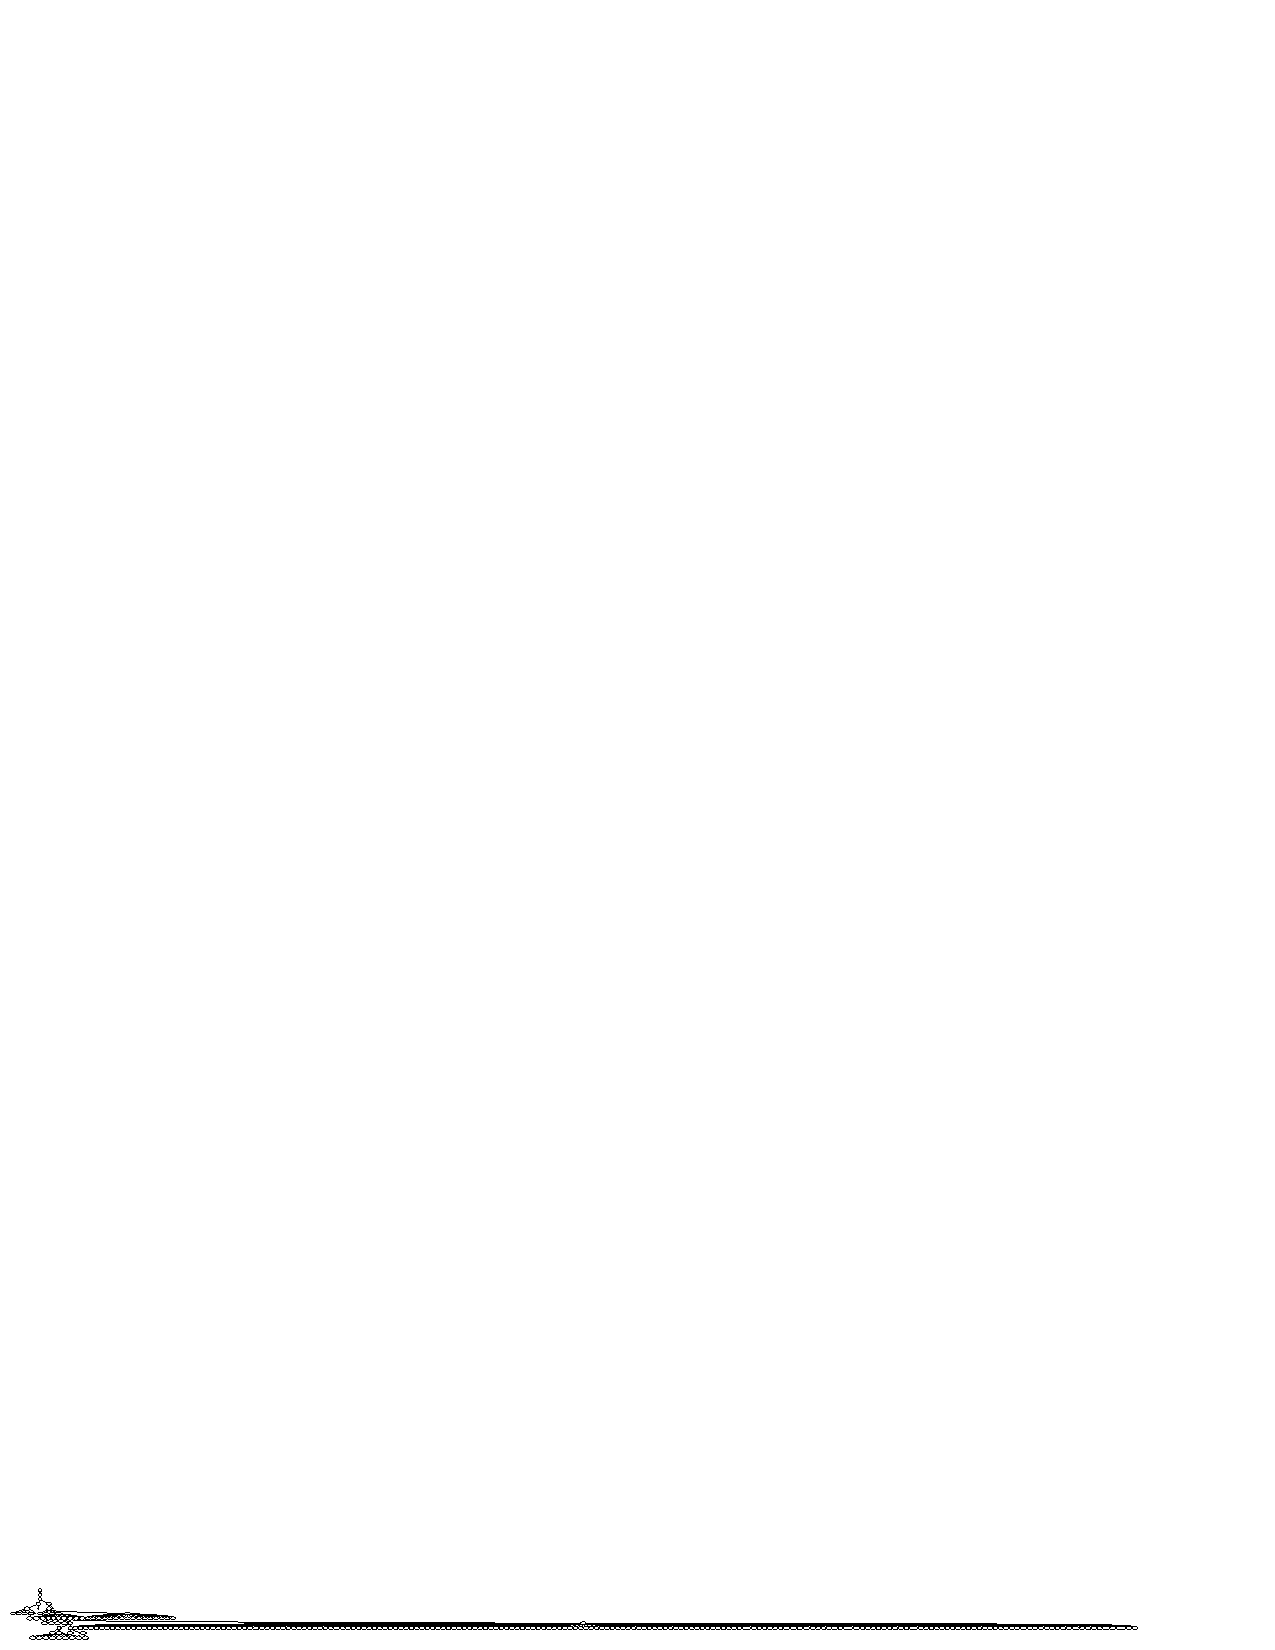
\includegraphics[scale=0.50]{\TopSourceDirectory/docs/Rose/asm_code_samples_gcc}
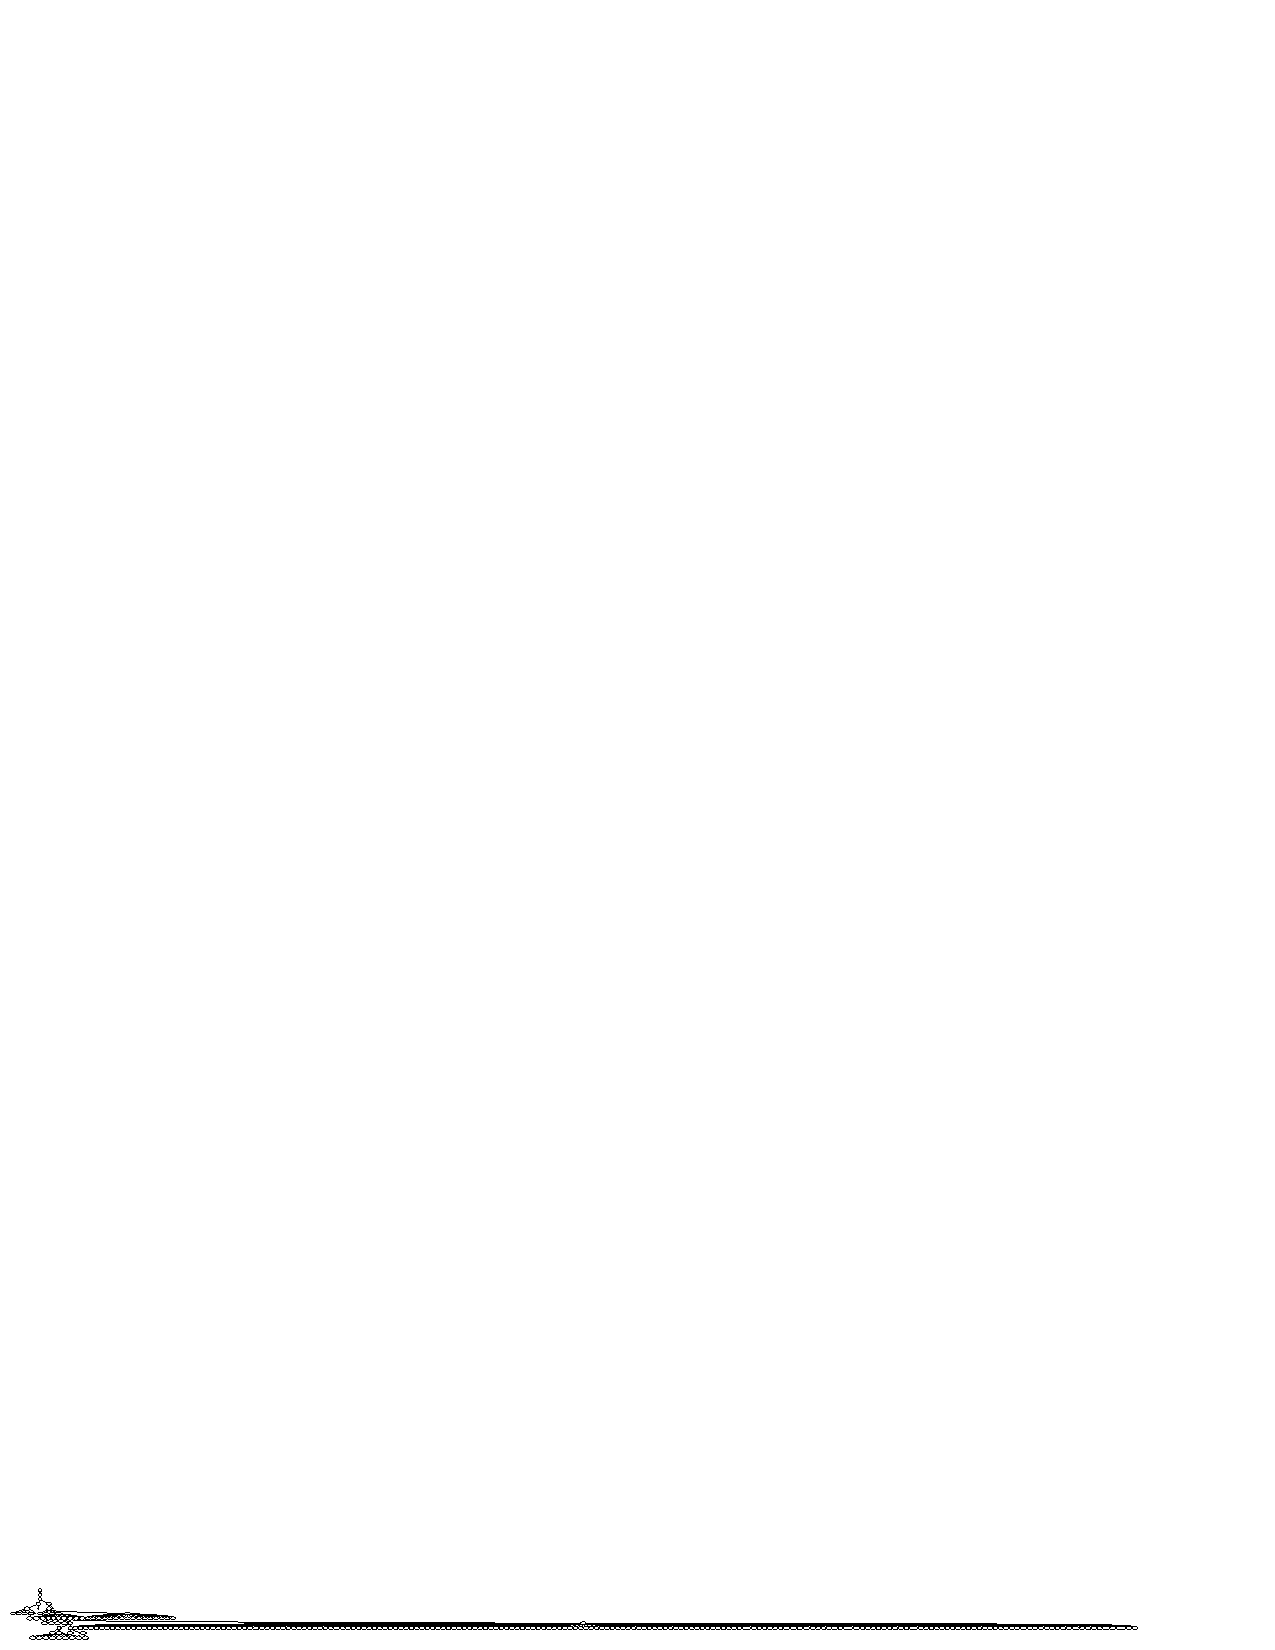
\includegraphics[,viewport=5 1 100 30,scale=2]{\TopSourceDirectory/docs/Rose/asm_code_samples_gcc}
\caption{The AST for a PE (Windows) binary executable (binary file format only), with long
    list of symbols (half of which are clipped on the right side of the image).} 

\label{binaryAnalysis:BinaryExecutableFormatAST_1}
\end{figure}

Figure \ref{binaryAnalysis:BinaryExecutableFormatAST_1} shows the graph of the AST
formed by just the binary file format (sections, symbols, etc.).  This figure shows
the different IR nodes used to represent the binary file format (without the disassembled 
instructions, in this case) and the large list of symbols within the symbol table (the 
long list that is partially truncated on the right edge of the figure).
This graph is quite large and does not fit well on the page, the next figure
\ref{binaryAnalysis:BinaryExecutableFormatAST_2} shows a clipped image with more detail.


\begin{figure}
% \includegraphics[angle=90,scale=0.75,width=5in,height=1in]{\TopSourceDirectory/src/frontend/ExecFormats/BinaryFileFormat}
\includegraphics*[angle=90,viewport=5 1 40 30,scale=18]{\TopSourceDirectory/docs/Rose/asm_code_samples_gcc}
\caption{The CROPPED AST for a PE (Windows) binary executable (binary file format only).} 

\label{binaryAnalysis:BinaryExecutableFormatAST_2}
\end{figure}

Figure \ref{binaryAnalysis:BinaryExecutableFormatAST_2} shows a cropped view of the graph
of the AST formed by just the binary file format (sections, symbols, etc.).  This figure
shows two {\em SgAsmInterpretation} IR nodes; this is a Windows PE binary and all windows
PE binaries contain both a 16-bit MS-DOS header (and some 16-bit code) and a 32-bit Windows
PE header (with sections that have 32-bit code); thus there are two SgAsmInterpretation IR
nodes (one for the 16-bit interpretation of the instructions and one for the 32-bit 
interpretation of the instructions).  Note that ELF format files will have only one
SgAsmInterpretation IR nodes (because there is only a single interpretation possible), but
other file formats can contain many interpretations; formed form a composite of code to
support wide ranges of portability.

*Note: The actually file used is in these figures is: {\tt ROSE/docs/Rose/asm\_code\_samples\_gcc.pdf}.

\subsection{Instruction Disassembly}
% NOTE: This subsection comes almost verbatim from the doxygen documentation in Disassembler.h

ROSE has its own disassembler (for x86, ARM, and PowerPC); a recursive disassembler that is well suited to details of variable
length instruction set handling and data stored in the instruction stream.  All details of the instructions, and the operands
and operator expression trees, etc. are stored in the binary AST as separate IR nodes.  The SgAsmInstruction class and its
architecture-specific subclasses represent individual instructions. The arguments for those instructions are represented by the
SgAsmExpression class and subclasses thereof.
\fixme{We need an example of the AST for a few instructions.}

Disassembly normally happens automatically unless the {\tt -rose:read\_executable\_file\_format\_only} switch is specified.
Alternatively, this Disassembler class can be used to explicitly disassemble parts of a file. The Disassembler class
handles all non-architecture-specific details of disassembly, such as where to search for instructions in the address
space and how instructions are concatenated into basic blocks.  The Disassembler has a pure virtual method,
disassembleOne, that is implemented by architecture-specific subclasses and whose purpose is to disassemble one
instruction.

New architectures can be added to ROSE without modifying any ROSE source code. One does this by subclassing an existing
disassembler, overriding any necessary virtual methods, and registering an instance of this subclass with the
{\tt Disassembler::register\_subclass} method.  If the new subclass can handle multiple architectures then a disassembler is
registered for each of those architectures.

When ROSE needs to disassemble something, it calls {\tt Disassembler::lookup}, which in turn calls the {\tt can\_disassemble}
method for all registered disassemblers.  The first disassembler whose {\tt can\_disassemble} returns true is used for the
disassemby.

If an error occurs during the disassembly of a single instruction, the disassembler will throw an exception. When
disassembling multiple instructions the exceptions are saved in a map, by virtual address, and the map is returned to the
caller along with the instructions that were successfully disassembled.

The main interface to the disassembler is the {\tt disassembleBuffer} method. It searches for instructions based on the
heuristics specified in the {\tt set\_search} method, reading instruction bytes from a supplied buffer.  A MemoryMap object is
supplied in order to specify a mapping from virtual address space to offsets in the supplied buffer. The
{\tt disassembleBuffer} method is used by methods that disassemble whole sections, whole interpretations, or whole files; in
turn, it calls {\tt disassembleBlock} which disassembles sequential instructions until a control flow branch is encountered.

A MemoryMap object can be built that describes the entire virtual address space and how it relates to offsets in the
executable file.  This object, together with the entire contents of the file, can be passed to the {\tt disassembleBuffer}
method in order to disassemble the entire executable in one call.  However, if the executable contains multiple
independent interpretations (like a PE file that contains a Windows executable and a DOS executable) then the best
practice is to disassemble each interpretation individually.  The {\tt disassemble} method is convenient for this.

While the main purpose of the Disassembler class is to disassemble instructions, it also needs to be able to group those
instructions into basic blocks (SgAsmBlock) and functions (SgAsmFunction). It uses an instance of the
Partitioner class to do so.  The user can supply a partitioner to the disassembler or have the disassembler create a
default partitioner on the fly.  The user is also free to call the partitioner directly on the InstructionMap object
returned by most of the disassembler methods.

\subsection{Instruction Partitioning}
% NOTE: This subsection comes almost verbatim from the doxygen documentation in Partitioner.h

While the main purpose of the Disassembler class is to disassemble instructions, it also
needs to be able to group those instructions into basic blocks (SgAsmBlock) and functions
(SgAsmFunction). It uses an instance of the Partitioner class to do so.  The
user can supply a partitioner to the disassembler or have the disassembler create a
default partitioner on the fly.  The user is also free to call the partitioner directly
on the InstructionMap object returned by most of the disassembler methods.

When grouping instructions into basic blocks, the partitioner looks at the instruction
type and known successor addresses. A known successor address is a virtual address where
the processor will disassemble and execute the next instruction. Unconditional branch
instructions typically have a single known successor (the branch target); conditional
branches usually have two successors (the following, or fall-through, address and the
branch target); data processing and testing instructions have one successor (the
following address); and interrupt-causing instructions have no known successors. A branch
to a calculated (non-immediate) address does not qualify as a known successor. The
SgAsmInstruction's terminatesBasicBlock virtual method is used to make this
determination.

Once instructions are assigned to basic blocks, the partitioner assigns the basic blocks
to functions using a variety of heuristics, the set of which is determined by the values
specified in the Partioner's {\tt set\_heuristics} method. These are documented in the
SgAsmFunction class (see the FunctionReason enumeration).  When a function is
created, its {\tt reason} attribute will contain a bit vector describing which heuristics
detected this function.

\subsection{Dwarf Debug Support}
% NOTE:

   ROSE can now read the Dwarf debug information stored into binary executables (ELF only
at this point). This information is represented as Dwarf specific IR nodes in the AST and
thus can be optionally used (when it is available in the binary) as part of any binary 
analysis.  Only a few sections are supported at present: {\em .debug\_info},
{\em .debug\_line}, etc.  The dwarf support in ROSE uses {\em libdwarf} and is enabled in
ROSE using a configuration option: {\tt (configure --with-dwarf={\em<path to libdwarf>}}.
Note that {\em libdwarf} is optional, must be separately installed by the user, and
thus is obviously not distributed within ROSE.  
% The future of the Dwarf support in ROSE is not clear, 
We anticipate the Dwarf information in the AST to be useful for performance tools that
operate on the binary executable when the binary executable has been generated to include 
Dwarf debug information.

\fixme{Consider moving the Dwarf support from {\em src/frontend/SageIII} to
       {\em src/frontend/BinaryDisassembly} instead.}

\section{Binary Analysis}

   A number of binary analysis passes are provided, most are a part of the Compass
framework for software analysis.  See the {\em Compass User Manual} for more details on
supported binary analysis.

   The ROSE tutorial shows a number of binary analysis passes over both the binary
instructions and the executable file format.

\section{Compass as a Binary Analysis Tool}

   Compass is a tool framework for building software analysis tools using rules (on source
code and alternatively directly on binary executables). Compass
reports violations of the rules in the evaluation of the software.  Compass is a
relatively simple application built on top of ROSE.  Most of the complexity and code 
within Compass is that it includes a large collection to rules, each rule has its
own implementation of an arbitrary test over the source code or the binary.  Rules
(checkers) may be defined over the AST or any other graph built within ROSE to store 
program analysis information. See the Compass manual for more details on supported
binary analysis.  The ability to perform analysis of binary executables using Compass 
makes no assumptions that it is compiled with any specific options or that it contains
debug information, symbols, etc.


\section{Static Binary Rewriting}
   As part of general research on transformations of binaries (separate from analysis)
a number of techniques have been developed to support classes of transformations.
This static rewriting of the binary permits the development of performance tools 
that could support the analysis and rewriting of binaries for support of High 
Performance Computing (HPC). A principal focus is on IBM BGL and Cray XT support 
(DOE Office of Science supercomputers).

\subsection{Generic Section/Segment Modifications}
%===============================================================================================================================
%Generic Section/Segment Modifications
%===============================================================================================================================

\subsubsection{1a. Section/Segment file address shifting (low-level)}

   The low-level movement of an ELF Section or Segment within the file address space is performed with
   SgAsmGenericSection::set\_offset.  It changes the location of the section in the file and updates all relative virtual
   addresses (RVAs) that were primarily associated with the moved section.

   The main problems with this function are that it doesn't take into account the file locations of other sections, the file
   alignment constraints of the moved section, or the memory mapping. Specifically, after calling this function to move {\bf.text}
   one byte later in the file:
\begin{itemize}
   \item {\bf.text} might not satisfy its file alignment constraint.

   \item The end of {\bf.text} might overlap with the following section. The ELF unparser has undefined behavior when two sections
     overlap without storing identical bytes at the overlapping regions.

   \item {\bf.text}, if memory mapped (which it surely is), might not be consistent with the mapping of other adjacent or overlapping
     sections. For instance, {\bf.text} is contained in "ELF Load Segment 2" both in the file address space and in the mapped
     memory space. The offset from ELF Load Segment 2 to {\bf.text} must be identical in both file and memory.

   \item RVAs that point to instructions in {\bf.text} can be associated with the {\bf.text} section or with ELF Load Segment 2,
     depending on how they were parsed. Normally it doesn't matter which since the relationship between file address space and
     memory address space is consistent. But if you change the file addresses without changing memory addresses then the byte
     to which the RVA points could be ambiguous.
\end{itemize}

   Changes to ELF Section or Segment file addresses are reflected in the ELF Section Table and/or ELF Segment Table. If the
   particular SgAsmGenericSection is present in both tables then modifying its file address will result in updates to both
   tables.

   NOTE: Do not modify section offsets and sizes by modifying the section table entries. Changes to these values will be
   overwritten with actual, current section offsets and sizes when the section table is unparsed:
\begin{itemize}
	\item SgAsmElfSectionTableEntry::set\_sh\_offset
	\item SgAsmElfSectionTableEntry::set\_sh\_size
	\item SgAsmElfSectionTableEntry::set\_sh\_addr
\end{itemize}

   NOTE: Do not modify segment offsets and sizes by modifying the segment table entries. Changes to these values will be
   overwritten with actual, current segment offsets and sizes when the segment table is unparsed:
\begin{itemize}
   \item SgAsmElfSegmentTableEntry::set\_offset
   \item SgAsmElfSegmentTableEntry::set\_filesz
   \item SgAsmElfSegmentTableEntry::set\_vaddr
   \item SgAsmElfSegmentTableEntry::set\_memsz
\end{itemize}

\subsubsection{1b. Section/Segment file address shifting (high-level)}
   
   The SgAsmGenericFile::shift\_extend method is the preferred way to make minor offset and/or size adjustments to an ELF
   Section or Segment. It is able to shift a section to a high file and/or memory address and/or extend the segment:
\begin{itemize}
   \item It takes into account all sections in the file, adjusting their offsets and/or sizes accordingly.

   \item Sections to the right of the the section in question (Sq) are shifted upward to make room and prevent overlaps.

   \item Sections overlapping with Sq are extended to contain all of what they previously contained.

   \item The shift amounts are adjusted to satisfy alignment constraints of all affected sections.

   \item Unreferenced areas of the file can optionally be utilized as unused address space.

   \item Adjusting file address spaces also adjusts the memory address spaces in a compatible manner.
\end{itemize}

   NOTE: Do not modify section offsets and sizes by modifying the section table entries. Changes to these values will be
   overwritten with actual, current section offsets and sizes when the section table is unparsed:
\begin{itemize}
	\item SgAsmElfSectionTableEntry::set\_sh\_offset
	\item SgAsmElfSectionTableEntry::set\_sh\_size
	\item SgAsmElfSectionTableEntry::set\_sh\_addr
\end{itemize}

   NOTE: Do not modify segment offsets and sizes by modifying the segment table entries. Changes to these values will be
   overwritten with actual, current segment offsets and sizes when the segment table is unparsed:
\begin{itemize}
   \item SgAsmElfSegmentTableEntry::set\_offset
   \item SgAsmElfSegmentTableEntry::set\_filesz
   \item SgAsmElfSegmentTableEntry::set\_vaddr
   \item SgAsmElfSegmentTableEntry::set\_memsz
\end{itemize}

\subsubsection{2a. Section/Segment resizing (low-level)}

   The size of an ELF Section or Segment can be modified by calling SgAsmGenericSection::set\_size (for file size) and
   set\_mapped\_size (for mapped memory). However, this is a low-level interface that doesn't take into account other sections in
   the same file.  The preferred way to resize a section is with SgAsmGenericFile::shift\_extend.

   NOTE: For many kinds of sections, making the section larger will create an unreferenced area ("internal hole") at the end of
   the section. Other sections will automatically do something with the new address space (e.g., SgAsmElfStringSection will
   add the new address space to its free list).

\subsubsection{2b. Section/Segment resizing (high-level)}

   The preferred way to extend a section is to call SgAsmGenericFile::shift\_extend, which extends sections that contain the
   resized-section and shifts sections that are right (higher address) of the resized-section.  This function also takes into
   account alignment constraints, memory address space, and (optionally) holes in the address space.

\subsection{Modifications to the ELF File Header}
%===============================================================================================================================
%Modifications to the ELF File Header
%===============================================================================================================================

\subsubsection{1. Entry Point RVA}

   The entry RVA stored in the ELF File Header is adjusted whenever the section into which it points is moved in memory. It is
   also possible to adjust this address explicitly by modifying the first (and only) entry in SgAsmGenericHeader::entry\_rvas.

   NOTE: An RVA (rose\_rva\_t) is an offset with respect to the beginning of some section. If the section starting memory address
   changes then the RVA implicitly changes (RVA's are virtual addresses relative to some format-wide base address). Multiple
   sections can be mapped to the same memory (e.g., {\bf.text} and {\bf ELF Load Segment 2} are typically overlap in memory), but
   since an RVA is associated with only one section, modifying the other section(s) has no effect on the RVA even if the RVA
   happens to be inside the other sections as well.

   NOTE: The binding between an RVA and a section can be modified with rose\_rva\_t::set\_section. In fact, the link can be
   completely broken by passing a null section pointer, in which case the RVA is not relative to any section.

\subsubsection{2. File Format Byte order}

   File byte order can be changed by modifying the SgAsmGenericFormat object pointed to by the file header:

      SgAsmGenericHeader *fhdr = ....;
      fhdr->get\_exec\_format()->set\_sex(ORDER\_MSB);

   NOTE: Modifying the byte order affects only those sections that are actually parsed. If the ELF file contains a section
   whose purpose we don't recognize then the original section data is written to the new file.

\fixme{If the byte order is not specified in the ELF header (e\_ident\_data\_encoding other than 1 or 2) then the parser will
   make an educated guess and assign a byte order.  The unparsed file will differ from the original in this case at the sixth
   byte of the file.}

\subsubsection{3. ELF Word Size}

   File word size can be changed between 4 bytes and 8 bytes by modifying the SgAsmGenericFormat object pointed to by the file
   header:

      SgAsmGenericHeader *fhdr = ....;
      fhdr->get\_exec\_format()->set\_word\_size(4);

   When changing word sizes, any fields that have values too large to represent in the new word size will cause the unparser
   to abort.

   NOTE: Modifying the word size affects only those sections that are actually parsed. If the ELF file contains a section whose
   purpose we don't recognize then the original section data is written to the new file.

\fixme{Increasing word size probably requires allocating more space for many of the sections. Vice versa for decreasing the
   word size.}

\subsubsection{4. ELF Header Magic Number}

   An ELF header has a four-byte magic number, usually 0x7f, 'E', 'L', 'F'.  The magic number can be modified by changing the
   string from SgAsmGenericHeader::get\_magic.  It must be exactly four characters in length.

\subsubsection{5. ELF File Purpose (lib, executable, core, etc.)}

   The file purpose should be modified by setting two fields, using

\begin{enumerate}
      \item SgAsmElfFileHeader::set\_p\_e\_type
      \item SgAsmGenericFormat::set\_purpose
\end{enumerate}

   Both members should be set to compatible values. The former is the value from the ELF specification and the latter is a
   constant: PURPOSE\_UNSPECIFIED, PURPOSE\_LIBRARY, PURPOSE\_EXECUTABLE, PURPOSE\_CORE\_DUMP, PURPOSE\_PROC\_SPECIFIC, PURPOSE\_OTHER.

\fixme{set\_p\_e\_type should probably call set\_purpose, but we can't go the other direction because the mapping is N:1.}

\subsubsection{6. ELF Version}

   To change the ELF version assign a new value by calling set\_version on the object returned by
   SgAsmGenericHeader::get\_exec\_format.  This doesn't have any effect on the code generated by the unparser since the parser
   only knows about ELF format 1.
   
\subsubsection{7. ELF Target Architecture}

   Modify the target architecture by calling two functions:

       SgAsmElfHeader::set\_e\_machine -- sets the ELF specific value
       SgAsmGenericHeader::set\_isa   -- sets the generic value

   You should call both with consistent values.

\subsubsection{8. ELF Section or Segment Table location}

   The SgAsmElfFileHeader::set\_e\_shoff and set\_e\_phoff methods have been removed since calling them had no lasting effect
   anyway. Instead, if you want to change one of these values for unparsing, then modify the actual SgAsmGenericSection that
   holds the table (e.g., calling SgAsmGenericFile::shift\_extend).

\subsubsection{9. ELF Section or Segment Table size}

   The number of entries in the section or segment table cannot be modified by calling set\_e\_shnum or set\_e\_phnum on the
   SgAsmElfFileHeader \fixme{Remove these functions.}. Rather, the sizes are obtained by looking at what sections and segments
   are currently defined and writing an entry to the file for each one.

\subsubsection{10. ELF Section Names}

   Elf section names can be modified. Doing so may cause extensive changes to the executable due to reallocation of the section
   holding the string table.

   Do not call SgAsmElfSectionTableEntry::set\_sh\_name since that value will be overwritten based on the actual, current
   location of the name in the associated string table.

\subsubsection{11. ELF Segment Names}

   ELF segment names are often parser-generated based on constants in the ELF Segment Table. However, if the segment
   corresponds to an actual ELF Section defined in the ELF Section Table then the segment and section share the same
   SgAsmGenericSection object and changing the name causes the ELF Section name to change with no effect on the segment table.

\subsubsection{12. ELF Section Name Table}

   The section that holds the section names is identified in the ELF File Header (get\_e\_shstrndx). Although it is possible to
   change this value, doing so will have no effect on the currently-defined sections: they will continue to use the original
   string table for their names.

\subsection{Modifications to ELF String Tables and their Containing Sections}
%===============================================================================================================================
%Modifications to ELF String Tables and their Containing Sections
%===============================================================================================================================

\subsubsection{1. Move/Extend}

   See SgGenericFile::shift\_extend.  When a string table is extended the new address space is added to the table's free list.

\subsubsection{2. New String}

   A new string can be created by calling the SgAsmStoredString allocator and passing a string table (something derived from
   SgAsmGenericStrtab) and the initial string value.  The string is not actually allocated space in the file until the new file
   is unparsed or until someone calls SgAsmStoredString::get\_offset.

\subsubsection{3. Value modification}

   A string can be modified by assigning a new value via SgAsmStoredString::set\_string. Storage is not allocated for the new
   value until the AST is unparsed or someone calls SgAsmStoredString::get\_offset.  The previous value is freed.

\subsubsection{4. Shared strings}

   Three forms of sharing are supported:

\begin{enumerate}
   \item Two objects (section names, symbol names, etc) share the same string and changing one string causes the other to change
      as well. This kind of sharing is not typically encountered in ELF although the underlying string table classes support
      it.

   \item Two objects have independent strings that happen to have the same value and point to the same offset in the string
      table. In this case, changing one string doesn't change the other. This kind of sharing is often encountered in ELF.

   \item Two objects have independent strings and one is an ending substring of another (e.g., "main" and "domain"). Changing one
      string does not affect the other. This kind of sharing is also common in ELF.
\end{enumerate}

\subsubsection{5. String table internal holes}

   If a sequence of bytes in a string table is not referenced by anything known to the parser, then those bytes are marked as
   internal holes and are prevented from moving with respect to the beginning of the string table. Internal holes are not
   placed on the string table free list (because something we didn't parse might be pointing to them).  The internal holes are
   available with SgAsmGenericSection::congeal.

\subsubsection{6. Reallocation of all strings}

   A string table can be repacked by freeing all it's strings and then reallocating.  We can reallocate around the internal
   holes or through the internal holes.

       strtab.free\_all\_strings();   /* free\_all\_strings(true) blows away internal holes */
       strtab.reallocate();

   The ELF allocator will do its best to overlap storage (e.g., "domain" overlaps with "main").

\subsubsection{7. Deletion of a string}

   A string is deleted by changing its value to the empty string.

\subsubsection{8. Stored strings vs. non-stored strings.}

   If a string value has storage space in a file (such as an ELF Section name), then it's an instance of
   SgAsmStoredString. Otherwise the string is either an std::string or SgAsmBasicString. SgAsmBasicString and SgAsmStoredString
   both derive from SgAsmGenericString.  Changing the value of an SgAsmBasicString has no effect on the unparsed file.

\subsection{Modifications ELF Section Table Entries}
%===============================================================================================================================
%Modifications ELF Section Table Entries
%===============================================================================================================================

Every ELF Section defined by the ELF Section Table is parsed as an SgAsmElfSection, which is derived from SgAsmGenericSection.
The SgAsmElfSection::get\_section\_entry returns a pointer to the ELF Section Table Entry (SgAsmElfSectionTableEntry). Some
members of these objects can be modified and some can't.

\subsubsection{1. These functions should not be called since their values are overwritten during the unparse phase:}

\begin{itemize}
   \item SgAsmElfSectionTableEntry::set\_sh\_name   -- see SgAsmGenericSection::set\_name
   \item SgAsmElfSectionTableEntry::set\_sh\_addr   -- see SgAsmGenericFile::shift\_extend
   \item SgAsmElfSectionTableEntry::set\_sh\_offset -- see SgAsmGenericFile::shift\_extend
   \item SgAsmElfSectionTableEntry::set\_sh\_size   -- see SgAsmGenericFile::shift\_extend
   \item SgAsmElfSectionTableEntry::set\_sh\_link   -- don't call (no alternative yet)
\end{itemize}
   
\subsubsection{2. Can modify}

\fixme{What text should go here?}

\begin{itemize}
   \item SgAsmElfSectionTableEntry::set\_sh\_type
   \item SgAsmElfSectionTableEntry::set\_sh\_flags, although the Write and Execute bits are ignored
   \item SgAsmElfSectionTableEntry::set\_sh\_info      \fixme{Is this complete?}
   \item SgAsmElfSectionTableEntry::set\_sh\_addralign \fixme{Is this complete?}
   \item SgAsmElfSectionTableEntry::set\_sh\_entsize   \fixme{Is this complete?}
\end{itemize}


\section{Dynamic Analysis Support}
\label{intel_pin}

   Recent work in ROSE has added support for dynamic analysis and for mixing of dynamic
and static analysis using the Intel Pin framework. This optional support in ROSE
requires a configure option ({\tt --with-IntelPin=$<path$>}.  The {\tt path} in
the configure option is the path to the top level directory of the location of
the Intel Pin distribution.  This support for Intel Pin has only been tested
on a 64bit Linux system using the most recent distribution of Intel Pin (version 2.6).

Note: The dwarf support in ROSE is currently incompatible with the dwarf support in
Intel Pin.  A message in the configuration of ROSE will detect if both support for
Dwarf and Intel Pin are both specified and exit with an error message that they
are incompatible options.


\section{Usage}
     See the ROSE Tutorial for examples.



